\chapter{Dataset}
\section{Struttura del dataset}
Il dataset è composto da un set di $3762$ immagini, ognuna delle quali è stata
ottenuta dalla risonanza magnetica del cervello. Ad ogni immagine è stata
associata un etichettata la quale permette di rappresentare la presenza o meno
di un tumore al cervello. Nel dataset è presente una colonna, \textit{Class},
nella quale sono presenti le etichette, ovvero:
\begin{itemize}
    \item \textbf{Presenza del tumore}: $T = 1$
    \item \textbf{Assenza del tumore}: $T = 0$
\end{itemize}

Oltre alla colonna \textit{Class}, il dataset è composto da altre $13$ colonne,
nelle quali sono presenti le feature calcolate sulle immagini. Tali sono state
ottenute calcolando i \textbf{momenti Hu} sulle immagini della risonanza magnetica.
I momenti Hu catturano le informazioni di base sull'immagine come l'area
dell'oggetto, il centroide, l'orientamento e altre proprietà.

Gli attributi di cui è composto il dataset possono essere suddivisi in 2 gruppi\cite{explanation-features}:
\begin{enumerate}
    \item \textbf{First Order Features}: forniscono informazioni legate alle
          distribuzione dei livelli di grigio dell'immagine. Queste features
          corrispondono alle statistiche descrittive calcolate sui valori di
          ciascun pixel dell'immagine. Le statistiche descrittive calcolate sono:
          \begin{itemize}
              \item \textbf{Media}
              \item \textbf{Varianza}
              \item \textbf{Deviazione standard}
              \item \textbf{Indice di asimmetria}
              \item \textbf{Indice di kurtosis}
          \end{itemize}
    \item \textbf{Second Order Features}: forniscono informazioni a livello di
          composizione della texture dell'immagine.
          \begin{itemize}
              \item \textbf{Contrasto}: misura la variazione locale dei livelli
                    di grigio dei pixel. Maggiore sarà il valore allora maggiore
                    sarà il contrasto dell'immagine.
              \item \textbf{Energia}: misura l'eterogeneità o la variazione
                    dell'intensità dell'immagine. Più piccolo è il valore allora
                    meno variazioni di intensità e più omogenea sarà la texture,
                    al contrario, più la texture è irregolare allora maggiore
                    sarà il valore.
              \item \textbf{ASM}: misura quanto sono distribuiti uniformemente i
                    livelli di grigio nell'immagine. Più i livelli di grigio sono
                    uniformemente distribuiti minore sarà il valore dell'indice.
              \item \textbf{Entropia}: misura la randomicità dei livelli di
                    grigio, quindi più piccolo è il valore, più la texture
                    sarà uniforme.
              \item \textbf{Homogeneous}: misura secondaria del contrasto. Più
                    alto sarà l'indice allora minore sarà il contrasto dell'immagine.
              \item \textbf{Dissimilarity}: misura quanto spesso differenti
                    combinazioni dei valori di intensità dei pixel occorrono
                    nell'immagine. Un valore alto indica che l'immagine ha una
                    maggior variazione delle intensità dei pixel vicini,
                    quindi più complessa sarà la texture.
              \item \textbf{Correlation}: misura la correlazione tra pixel nelle
                    due diverse direzioni.
              \item \textbf{Coarseness}: misura quanto l'immagine è composta da
                    regioni di intensità omogenea, ovvero quanto è granulare o
                    fine la texture.
          \end{itemize}
\end{enumerate}
\section{Analisi descrittiva}
Il dataset è formato da un totale $3762$ istanze, ciascuna delle quali è descritta
da $15$ attributi così suddivisi:
\begin{itemize}
    \item $13$ rappresentano le feature calcolate sulle immagini della risonanza
          magnetica. Tutti questi attributi sono di tipo \textit{float}.
    \item $1$, ovvero l'attributo \textit{Image}, rappresenta l'identificativo
          dell'immagine a cui si riferisce l'istanza.
    \item $1$, ovvero l'attributo \textit{Class}, rappresenta l'etichetta associata
          all'immagine. Questo attributo è stato convertito da \textit{intero} a
          \textit{categorico} per poter effettuare la classificazione.
\end{itemize}

Caricato il dataset, è stato eseguito un controllo per verificare che non ci fossero
valori nulli. In questo caso non sono stati trovati valori nulli, quindi non è
stato necessario eseguire alcuna operazione per la gestione di tali valori.
% Todo: controllare se nel dataset ci sono valori duplicati

Successivamente, si è proceduto con il calcolo delle statistiche descrittive per
gli attributi numerici presenti nel dataset. Questa operazione ha permesso di
ottenere le informazioni riportate nella tabella \ref{tab:desc-stat}.

\begin{table}[!ht]
    \centering
    \resizebox{\textwidth}{!}{\begin{tabular}{|c|c|c|c|c|c|c|c|c|c|c|c|c|c|}
            \hline         & \textbf{Mean} & \textbf{Variance} & \textbf{Standard Deviation} & \textbf{Entropy} & \textbf{Skewness} & \textbf{Kurtosis} & \textbf{Contrast} & \textbf{Energy} & \textbf{ASM} & \textbf{Homogeneity} & \textbf{Dissimilarity} & \textbf{Correlation} & \textbf{Coarseness} \\ \hline
            \textbf{count} & 3762          & 3762              & 3762                        & 3762             & 3762              & 3762              & 3762              & 3762            & 3762         & 3762                 & 3762                   & 3762                 & 3762                \\
            \textbf{mean}  & 9.488890      & 711.101063        & 25.182271                   & 0.073603         & 4.102727          & 24.389071         & 127.961459        & 0.204705        & 0.058632     & 0.479252             & 4.698498               & 0.955767             & 7.458341e-155       \\
            \textbf{std}   & 5.728022      & 467.466896        & 8.773526                    & 0.070269         & 2.560940          & 56.434747         & 109.499601        & 0.129352        & 0.058300     & 0.127929             & 1.850173               & 0.026157             & 0.000000e+00        \\
            \textbf{min}   & 0.078659      & 3.145628          & 1.773592                    & 0.000882         & 1.886014          & 3.942402          & 3.194733          & 0.024731        & 0.000612     & 0.105490             & 0.681121               & 0.549426             & 7.458341e-155       \\
            \textbf{25\%}  & 4.982395      & 363.225459        & 19.058475                   & 0.006856         & 2.620203          & 7.252852          & 72.125208         & 0.069617        & 0.004847     & 0.364973             & 3.412363               & 0.947138             & 7.458341e-155       \\
            \textbf{50\%}  & 8.477531      & 622.580417        & 24.951560                   & 0.066628         & 3.422210          & 12.359088         & 106.737418        & 0.225496        & 0.050849     & 0.512551             & 4.482404               & 0.961610             & 7.458341e-155       \\
            \textbf{75\%}  & 13.212723     & 966.954319        & 31.095889                   & 0.113284         & 4.651737          & 22.640304         & 161.059006        & 0.298901        & 0.089342     & 0.575557             & 5.723821               & 0.971355             & 7.458341e-155       \\
            \textbf{max}   & 33.239975     & 2910.581879       & 53.949809                   & 0.394539         & 36.931294         & 1371.640060       & 3382.574163       & 0.589682        & 0.347725     & 0.810921             & 27.827751              & 0.989972             & 7.458341e-155       \\ \hline
        \end{tabular}}
    \caption{Statistiche descrittive degli attributi}
    \label{tab:desc-stat}
\end{table}

Questa operazione ha permesso di ottenere alcune informazioni sul dataset.
Innanzitutto, ha permesso di osservare che i valori associati agli attributi non
sono standardizzati dal momento che nessun dato ha media $0$ e deviazione
standard $1$.

La standardizzazione delle feature è stata fatta, utilizzando l'equazione
\ref{eq:std-features}, solo per le SVM e il modello neurale, mentre per Gaussian
Bayes la standardizzazione viene fatta in automatico dalla libreria del modello.
\begin{equation}
    F_{\mu, \sigma} = \frac{F - \mu}{\sigma}
    \label{eq:std-features}
\end{equation}

In aggiunta alle statistiche descrittive, per ogni feature si è realizzato un
istogramma attraverso il quale è stato possibile realizzare una prima analisi
visiva sulla distribuzione dei valori. Questa operazione è stata svolta per
verificare se le feature seguono una distribuzione normale.

\textbf{TODO:immagine}

Da questi grafici si evince che le feature \textit{Energy}, \textit{Homogeneity}
e \textit{Coarseness} non seguono una distribuzione normale, a differenza delle
altre feature che possono essere considerate normali. In ogni caso, anche se non
seguono l'ipotesi di normalità, si è deciso comunque di utilizzarli, anche se
stiamo andando contro le assunzioni dei modelli che vogliamo utilizzare. % TODO: non ho capito cosa vuol dire

Da questa analisi, è stato possibile osservare che la feature \textit{Coarseness}
assume valori molto bassi, quindi è stato pensato di convertire questa feature
ad una scala logaritmica, permettendo di aumentare la significatività dei valori.

Nonostante questa operazione, la feature \textit{Coarseness} presenta una deviazione
standard pari a circa $0.02$, valore non particolarmente significativo, quindi
questo ci ha permesso di escludere questa feature perché sicuramente non sarà la
feature più discriminante.

Oltre all'analisi descrittiva delle feature, è stato eseguito anche un analisi
sulle etichette, ovvero sulle classi. Questo è stato fatto per verificare se le
classi sono bilanciate, ovvero se il numero di esempi positivi è simile al numero
di esempi negativi.

In questo caso, realizzando un istogramma, riportato in figura \ref{fig:dist-classi},
che rappresenta le frequenze assolute delle classi. Da questo si può notare che 
la distribuzione di esse è bilanciate, infatti, circa il $55\%$ degli esempi sono 
negativi (assenza del tumore), contro circa il $45\%$ degli esempi sono positivi 
(presenza del tumore).

\begin{figure}[!ht]
    \centering
    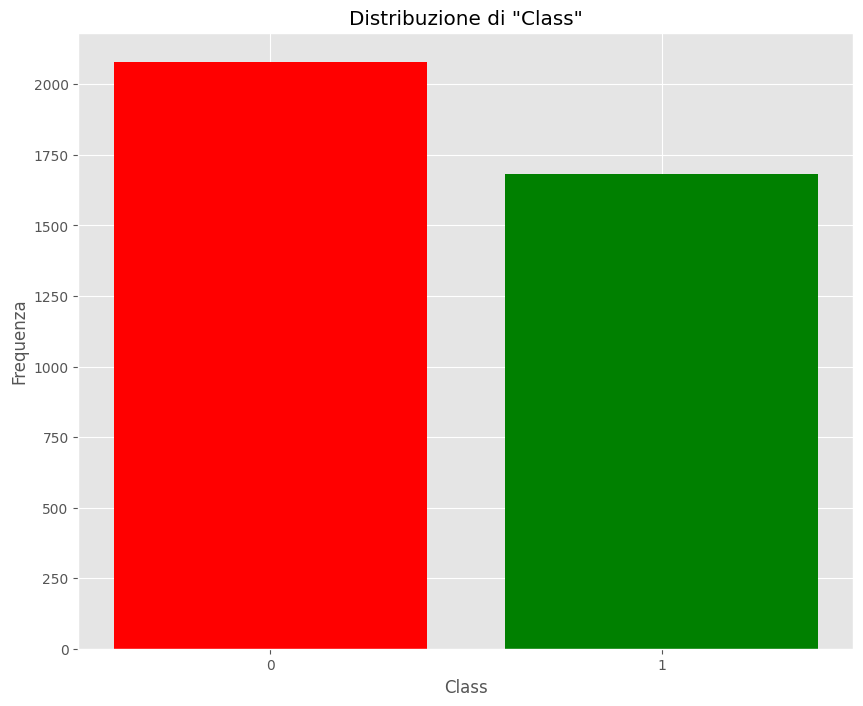
\includegraphics[width=0.5\textwidth]{img/analisi/distribuzioneClassi.png}
    \caption{Distribuzione delle classi}
    \label{fig:dist-classi}
\end{figure}

\textbf{Non è già stato detto prima?}
Successivamente risulta importante analizzare se le distribuzioni si avvicinano
ad una normale standard, di conseguenza sono stati disegnati i barplot delle frequenze
di ciascuna feature. Dai grafici si evince che tutte le feature eccetto \textit{Energy} e
\textit{Homogeneity} sono distribuite normalmente.

Dal barplot delle features creato precedentemente, si possono ottenere ulteriori
informazioni sulla distribuzione potenzialmente normale delle altre feature. Infatti,
la distribuzione della \textit{Standard deviation} è simmetrica, mentre tutte
le altre presentano una asimmetria.

Ricapitolando, da questo primo studio descrittivo è stato modificato il dataset
rimuovendo la feature \textit{Coarseness}.

\textbf{TODO:immagine}

\subsection{Analisi delle correlazioni}
Il passaggio successivo è  stato quello di analizzare le correlazioni tra le feature. 
Questo è stato fatto in modo tale da ridurre la dimensionalità dei dati, nello 
specifico sono state suddivise le feature in gruppi di feature altamente correlate 
tra loro, e in un secondo momento è stata scelta una feature per ogni gruppo.

Per fare ciò, è stata realizzata una matrice di correlazione, riportata in figura
\ref{fig:corr-matrix}, attraverso la quale è stato possibile osservare le correlazioni
tra le feature.

\begin{figure}[!ht]
    \centering
    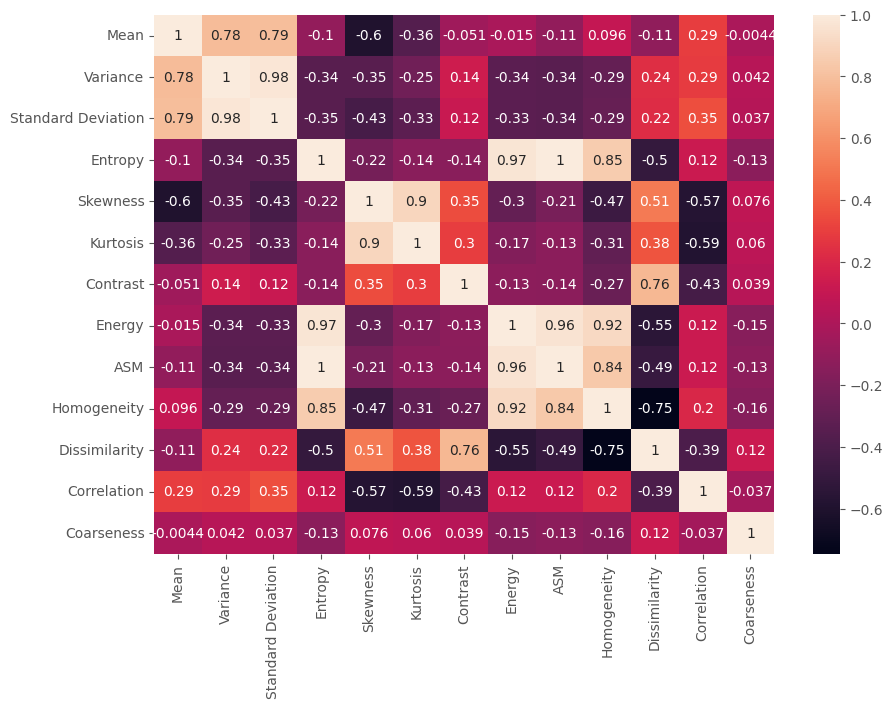
\includegraphics[width=0.5\textwidth]{img/analisi/corr.png}
    \caption{Matrice di correlazione}
    \label{fig:corr-matrix}
\end{figure}

Dall'analisi di questa matrice, si possono osservare diverse correlazioni tra le
feature. Innanzitutto, si può notare una forte correlazione positiva tra le feature
\textit{Mean}, \textit{Variance} e \textit{Standard deviation}. Questa correlazione
è facilmente spiegabile analizzando le immagini prodotte dalle risonanze magnetiche.
Infatti, essendo in bianco e nero, se la media tende a $1$ (colore bianco) allora
la varianza e la deviazione standard aumentano, perché sono presenti diversi 
pixel bianchi. Questo comporta che le transizioni dal nero assoluto al bianco
assoluto neccessitano di regioni di pixel maggiore rispetto ad una transizione
tra nero assoluto e grigio ($0.5$).

Invece, la correlazione tra varianza è deviazione standard facilmente spiegabile
perché la deviazione standard è la radice quadrata della varianza ($SD[P] = \sqrt{VAR[P]}$).

\textbf{TODO:immagine}

Una seconda forte correlazione positiva si può osservate tra le feature che 
misurano l'\textbf{uniformità dei livelli di grigio} dei pixel, più precisamente 
tra le feature \textit{Entropy}, \textit{ASM}, \textit{Homogeneity} ed 
\textit{Energy}. Queste feature quantificano delle informazioni legate alla
texture dell'immagine, quindi la forte correlazione positiva può essere spiegata 
analizzando le texture delle immagini su cui vengono calcolate. Più precisamente
se si ha un valore molto alto della feature \textit{Entropy}, significa che la
texture non è uniforme, ovvero si hanno strutture complesse e irregolari, quindi
meno uniforme sarà la distribuzione dei livelli di grigio, aumentando l'indice
di \textit{ASM}, comportando di conseguenza un aumento delle variazioni di intensità
dei livelli di grigio, aumentando di conseguenza anche l'indice di \textit{Energy},
infine, (\textbf{cosa c'entra Homogeneity?}).

Al tempo stesso, la matrice di correlazione evidenza una forte correlazione positiva
tra gli indici che misurano la \textbf{morfologia della distribuzione}, ovvero
le feature di \textit{Skewness} e \textit{Kurtosis}. Questa dipendenza implica il
fatto che più la distribuzione è leptokurtica (Kurtosis grande), ovvero la frequenza
dei livelli di grigio dei pixel si concentrano interamente vicino alla media/mediana/
moda, allora più grande sarà la Skewness, ovvero maggiore sarà la tendenza ad avere
frequenze di livelli di grigio più vicino al bianco (coda di destra più altra rispetto
alla coda di sinistra).

La matrice della correlazione evidenzia anche una correlazione positiva tra le
feature di \textit{Contrast} e \textit{Dissimilarity}, ovvero maggiore sarà il
contrasto e maggiore sarà la complessità della texture.

In aggiunta dalla matrice si evidenza che le features di \textit{Dissimilarity}
e \textit{Homogeneity} sono correlate negativo, ovvero maggiore sarà il contrasto
allora minore è la complessità della texture.

Dalla correlazione delle features è possibile ridurre la dimensionalità del dataset
considerando sono le seguenti features:
\begin{itemize}
    \item \textbf{Mean}
    \item \textbf{Entropy}
    \item \textbf{Skewness}
    \item \textbf{Contrast}
    \item \textbf{Correlation}
\end{itemize}
A puro scopo didattico è stato pensato di eseguire i modelli non solo sul dataset
semplificato eliminando le correlazioni, ma anche applicando l'algoritmo PCA.

\section{PCA}
Precedentemente è stato presentato un primo modo per ridurre la dimensionalità
dei dati basandoci sull'analisi delle correlazioni. In seguito, è stato pensato
di provare ad utilizzare un metodo di trasformazione delle feature per ridurre
la loro dimensionalità e successivamente analizzare i risultati ottenuti. La 
scelta sul metodo da utilizzare è ricaduta su PCA.

Per prima cosa è statao necessario comprendere quante componenti delle nuove
feature sono necessarie per avere la maggior parte della varianza spiegata. Per 
fare ciò sono state separate le features dalla classe di ciascun esempio,
successivamente è stato effettuato il fit della PCA sull'istanza di ciascun dato
e successivamente è stato plottato all'interno di uno scatter plot per ogni 
componente la sua percentuale di varianza spiegata.

\textbf{TODO:immagine del plotting della PCA}

Dallo scatter plot si evidenzia come con solo le prime 3 componenti, si riesce
a raggiungere un totale dell'$85\%$ di varianza spiegata sui dati. In questo modo
una volta eseguita la pca e applicata la trasformazione, si selezionano solo le
prime 3 componenti dei nuovi dati trasformati. 
In aggiunta, dal momento che abbiamo ridotto la dimensionalità dei dati a $3$ 
allora, aggiungendo anche la colonna target, si possono rappresentare all'interno
di uno scatter plot a $3$ dimensioni e si può notare come i dati sono separabili
tramite un iperpiano.

\textbf{TODO:immagine del plotting delle nuove componenti}
